% file siminos/froehlich/slice/singul.tex
% $Author$ $Date$

% \section{Slice {\sset}}
%	\label{sec:singul}

If  two patterns are close, their group orbits will be nearly parallel,
$\braket{\groupTan(\ssp)}{\sliceTan{}} \neq 0$, and for a smooth flow the
slice will be transverse to all group orbits of $\ssp$ in an open
neighborhood of the {\template} \slicep. However, looking back at
\refeq{SL:CLEsliceRot} and \refeq{eq:so2reduced}, we see that the
\mslices\ introduces singularities in the \reducedsp. Two hyperplanes are
associated with  any given {\template} \slicep; the slice \refeq{PCsectQ0},
and the hyperplane of points \sspSing\ such that
\( %beq
\braket{\groupTan(\sspSing)}{\sliceTan{}}
 =
\braket{\sspSing}{\Lg^2\slicep}
 =0
%\,.
\) % ee{sliceSingl}
(for simplicity, in this section we specialize to the  $\SOn{2}$ case).
We shall refer to the $(d\!-\!2)$\dmn\ intersection of the two as
the {\em \sset} in the \reducedsp, $\sspRSing \in S \subset \pSRed$.
\beq
\braket{\groupTan(\sspRSing)}{\sliceTan{}}
 =
\braket{\sspRSing}{\Lg^2\slicep}
 =0
\,.
\ee{sliceSingl}
Just as the slice itself, the {\em \sset} goes through the origin.
For example, for \cLe\
$\sspRSing = (x_1^*,x_2^*,y_1^*,y_2^*,z)$,
$\sspRed = (x_1',x_2',y_1',y_2',z)$,
and the 3\dmn\ {\sset} $\sspRSing \in S$ in the \reducedsp\ is given by
\[
0 = {x_1^* x'_1+x_2^* x'_2+y_1^* y'_1+y_2^* y'_2}
\,.
\]
The {\sset} is purely an artifact of the particular choice of a
{\template}, and has nothing to do with the dynamics; the corresponding full
\statesp\ trajectory is smooth.

We show first that for the \mframes\ rotation angle $\gSpace$ the
singularity in \refeq{SL:CLEsliceRot} is only apparent, by computing it
for a trajectory that crosses the {\sset}. Next we show that if
$\ssp(\tau)$ is a smooth trajectory in full {\statesp}, then the
\reducedsp\ flow $\sspRed(\tau)$ jumps whenever it crosses the {\sset}
$\sspRSing$. We compute the size of the jump, and describe the behavior of nearby
trajectories.


Their crossings are
non-generic, but if we consider projections of successive instants of an
ergodic trajectory they can be approached arbitrarily closely.

At the
singular instant, the group tangent of a point $\sspRed=\LieEl^{-1} \ssp$
lies in the slice, $\braket{\groupTan(\sspRed)}{\sliceTan{}}$ is zero,
and neither the velocity $\dot{\gSpace}(\tau)$ along the group tangent
nor the velocity in the slice are defined.

At the instant of
coalescence the denominator in \refeq{SF:sliceEas} goes through a simple
pole, and the integrated trajectory within slice jumps.


not generic, but a computational and visualization nuisance

\subsection{Traversing {\sset}}
\label{sec:sliceSing}


Suppose the trajectory passes through a singularity at time
$\tau=\tau_0$, which we shall set to  $\tau_0=0$. $\ssp(\tau)$ is
$C^{\infty}$ since we can explicitly calculate any order derivative using
$\dot{\ssp}=\vel(\ssp)$. In the linear approximation the full \statesp\
trajectory near the singularity is given by
$\ssp(\tau)\simeq\hat{\ssp}+\vel(\hat{\ssp}) \tau$. Then apply the slice
condition \refeq{PCsectQ1} on $\gSpace(\tau)$ for each infinitesimal
generator $\sliceTan{a}$ of the Lie group at $\slicep$.
We can rotate the trajectory in the full {\statesp} so that $\hat{\ssp}$
is in the slice. This gives us the condition for $\gSpace$
\refeq{eq:slicecondition} in terms of the Taylor expansion
up to linear order:
\[
\braket{e^{\gSpace \cdot \Lg}(\hat{\ssp}+\vel(\hat{\ssp}) (\tau-\tau_0)+O(\tau^2))}
       {\sliceTan{a}} = 0
\,.
\]
If in addition we know that all the higher order terms in
the inner product are negligible compared to the linear term near $\tau_0$,
\beq
\braket{e^{\gSpace \cdot \Lg} O((\tau-\tau_0)^2)}{\sliceTan{a}}
\ll \braket{e^{\gSpace \cdot \Lg}\vel(\ssp(\tau))(\tau-\tau_0)}{\sliceTan{a}},
\ee{eq:neglig}
then we can take the limit of this expression as $\tau \rightarrow 0$:
\bea
\braket{e^{\gSpace \cdot \Lg}(\hat{\ssp}+\vel(\hat{\ssp}) \tau}{\sliceTan{a}}
    \continue
&\simeq& \braket{e^{\gSpace \cdot \Lg}\hat{\ssp}
    + e^{\gSpace \cdot \Lg}\vel(\hat{\ssp})\tau0}{\sliceTan{a}}
    \continue
&=&  \tau\braket{e^{\gSpace \cdot \Lg}\vel(\hat{\ssp})}{\sliceTan{a}}\approx 0
\,.
\eea
$\gSpace$ approaches $\gSpace^*$ such that $\braket{e^{\gSpace^* \cdot
\Lg}\vel(\hat{\ssp})}{\groupTan(\slicep)}= 0$ so $\gSpace$ approaches an
angle that rotates $\vel(\hat{\ssp})$ into the slice. Which angle it
approaches before and after the singularity depend on the restrictions
put on the moving frame, and the trajectory can
jump from one $\gSpace$ to another depending on this choice. The only
effect passing through a singularity will have on the \reducedsp\
trajectory then is to cause it jump from one point on a group orbit to
another at the singularity, and the trajectory will be smooth otherwise.
    \PC{set $\tau = 0$ at the singularity in \reffig{fig:dthetasing}}

% 2010-12-20 previously {CLEsingpass}{CLEnearsing2}
 \begin{figure}
 \begin{center}
(a)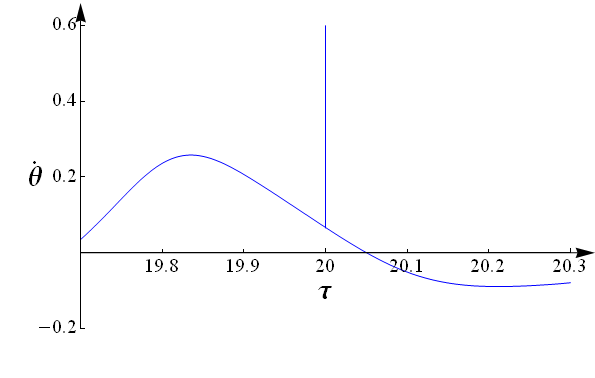
\includegraphics[width=0.45\textwidth]{dthetasing}%
(b)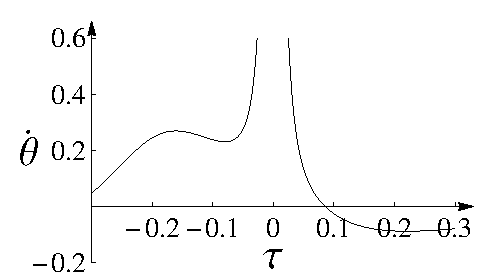
\includegraphics[width=0.45\textwidth]{dthetanearsing}%
 \end{center}
 \caption{\label{fig:dthetasing}
The {\groupVel} $\dot{\gSpace}$ for two \cLf\
\reducedsp\ trajectories in a slice defined by the {\template} $\slicep=(0.782?,-0.277?,-0.4?,0.12?,0)$:
 (a) As the trajectory $\sspRed(\tau)$ passes through the
{\sset} \refeq{sliceSingl}
%$\braket{\groupTan(\sspRed)}{\sliceTan{}}=0$
 at $\sspRSing=(-1.22?, ?3.212, -?4.31, ?1.11, ?4)$,
the {\groupVel} diverges
$\dot{\gSpace} \to \infty$ as a Dirac delta function.
(b) The {\groupVel} for a nearby trajectory going
through $\sspRSing+\delta \sspRed$,
where $\delta\sspRed=(0.01,0,0,0,0)$ exhibist a large
but finite excursion close to the singularity.
 }%
 \end{figure}

% 2010-12-20 previously {singpass}%
 \begin{figure}
 \begin{center}
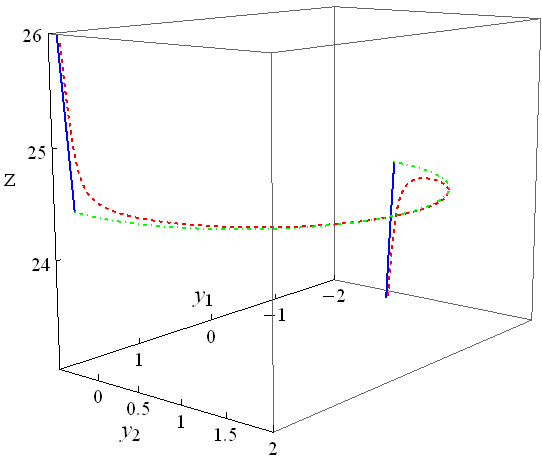
\includegraphics[width=0.45\textwidth]{singpass1}
 \end{center}
 \caption{\label{fig:singpass}
(color online).
Blow-up of the jump in \reffig{fig:Fullspace}\,(b).
(blue/dotted) A trajectory that passes through the singularity point
$\sspRSing=(-0.44, 3.23, -0.034, 6.37, 2.34)$ in the slice normal to
$\sliceTan{}=(-0.45, -1.05, 0.3, 0.5, 0.)$.
Note the jump in the trajectory,  caused by the divergence in
velocity (\reffig{fig:dthetasing}\,(a)) as the trajectory
passes through the singularity. The red/dashed trajectory has initial
point differing from the blue's by $(0,0,0.1,0,0)$, so it does not pass
through a singularity. The green trajectory is the group orbit of
$\sspRSing$ between the two $\gSpace$ that rotate $v(\sspRSing)$ in the
slice. Note also how the red/dashed trajectory begins near the
blue/dotted trajectory, closely follows the green trajectory after the
singularity point, reaches the other side of the blue/dotted arc and then
resumes closely following the blue/dotted trajectory.
 }%
 \end{figure}

\reffig{fig:dthetasing}


The {\groupVel} for two \cLf\
\reducedsp\ trajectories in a slice defined by the slice-fixing
point $\slicep=(0.782?,-0.277?,-0.4?,0.12?,0)$.
	\PC{move numerical values of \slicep\ from
	\reffig{fig:dthetasing} and \reffig{fig:singpass} captions
	to formulas in the main text. Explain where they come from}

As a trajectory $\sspRed(\tau)$ passes through the
{\sset} \refeq{sliceSingl}
the {\groupVel} diverges
$\dot{\gSpace} \to \infty$ as a Dirac delta function.

(b) The {\groupVel} for a nearby trajectory going
through $\sspRed+\delta \sspRed$,
where $\delta\sspRed=(0.01,0,0,0,0)$.


\reffig{fig:singpass}


%
% ****** End of file singul.tex ******
